%!TEX root = ../username.tex
\chapter{Results}
\hspace*{-0.187cm}This section will discuss how the two different approaches to artificial reverberation perform. It will begin by evaluating how the echo density of the Schroeder Comb Filter approach increases with the number of filters provided. Next, a comparison will be made between the Schroeder Comb Filter approach and the Convolution approach to determine how the purely artificial method compares to a reverb created from the Impulse Response of a real acoustic space. Finally, the chapter will end with where one can improve upon these designs and some of the drawbacks between the two approaches.

\section{Evaluating the Echo Density}
Each additional Comb Filter added to the reverberator in parallel increases the echo density linearly. With the aforementioned four Comb Filters, the echo density is 100. This figure can be increased with an implemented allpass filter in series within the reverberator. In doing so, the resulting echo density can be increased to the required 1000.

\begin{figure}[h] % [h] used to prevent {figure} from doing weird positioning
	\begin{center}
		\fbox{
		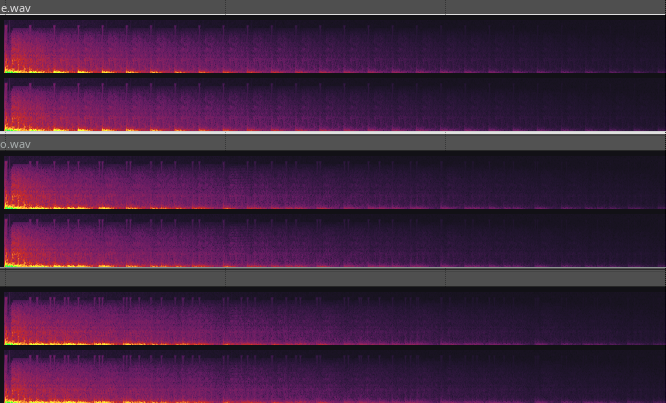
\includegraphics[width=12cm]{figures/Comb-Evaluations.png}
		}
		\caption{Several waveforms with a number of Comb Filters in parallel.}
	\end{center}
\end{figure}

With the short impulse provided as an input, the waveform visibly shows where each delay line repeats within the reverberator. While this can create an unwanted effect for lower echo densities, this problem is mitigated with instruments with a longer attack, such as a piano, or violin.

\section{Comparisons With a Real Acoustic Space}
Comparing this with the Convolution approach, one can ascertain that the Impulse Response provides a more realistic sound, but JUCE's DSP library prevents this from truly taking advantage of this in its current state. Once again, short impulse responses create regular peaks that can allow one to ascertain where exactly the delay line is repeating the given signal. However, this is likely due to the high performant requirements of this type of application, as the number of computations required increases exponentially the longer the Impulse Response provided is. While the current implementation is limited by the high performant requirements of the application, other reverberators using the same IR do provide highly convincing and realistic results, such as from ReaVerb.


\begin{figure}[h] % [h] used to prevent {figure} from doing weird positioning
	\begin{center}
		\fbox{
		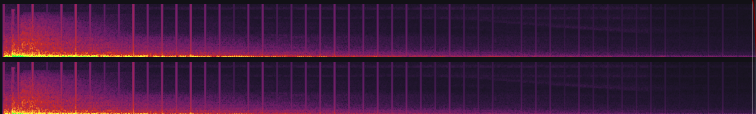
\includegraphics[width=14cm]{figures/Conv-Eval.png}
		}
		\caption{A waveform of a reverberated snare drum from a Convolved IR.}
	\end{center}
\end{figure}
